\subsection{Layers Tab}

The top half hosts the shared Layers Tree (see \nameref{sec:layers_tree}) augmented with Geographic-View-specific layer groups; the bottom half hosts the Item Mode panel (see \nameref{sec:geo_item_mode}), separated by a splitter.

\begin{figure}[H]
    \centering
    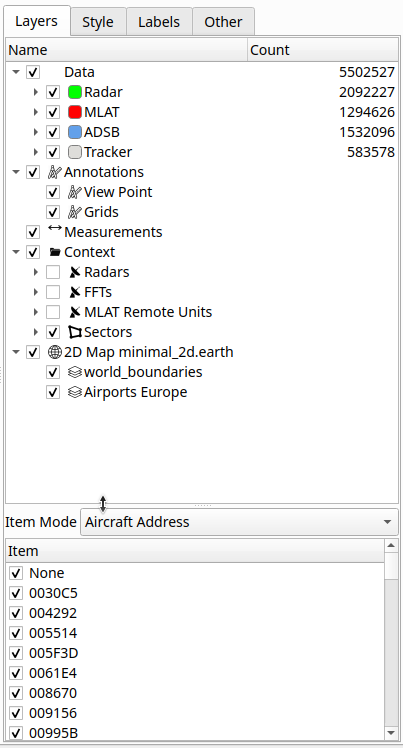
\includegraphics[width=8cm,frame]{figures/geoview_config_split.png}
  \caption{Geographic View: Layers tab splitter}
\end{figure}

The layer tree has the following top-level groups: \\

\begin{itemize}
 \item Data: Currently loaded DBContent, structured as in the shared Layers Tree
 \item Annotations: View annotations
 \item Measurements: Current distance measurements
 \item Context: Geographic content of the active Data Context (see \nameref{sec:configure_data_context})
 \begin{itemize}
  \item Radars
  \item FFTs
  \item MLAT Remote Units: one subgroup per MLAT Data Source (see \nameref{sec:ui_configure_ds_mlat_rus})
  \item Sectors
 \end{itemize}
 \item Map: Current map layers
\end{itemize}
 \ \\


\includegraphics[width=0.5cm]{../../data/icons/hint.png} For all data layers, a second column is shown, giving the count of number of target reports in the (sub-) layer (as were loaded from the database). \\

In the Layers widget, a number of operations are possible for each tree item.

\begin{table}[H]
  \center
  \begin{tabular}{ | l | l | l |}
    \hline
    \textbf{Operation} & \textbf{Trigger} &  \textbf{Description} \\ \hline
    View sub-items & Triangle & Opens or closes view of the sub-items \\ \hline
    Display item & Checkbox & Enables or disables display of items (and all sub-items) \\ \hline
    Display context menu & RMB Click on symbol & Opens the items context menu \\ \hline
  \end{tabular}
  \caption{Layer operations}
\end{table}

The context menu allows several actions to be performed on an item. If an item has sub-items, the same action will automatically be performed on the child items.

\subsubsection{Item Mode Panel}
\label{sec:geo_item_mode}

The Item Mode panel sits in the bottom and groups the loaded target reports by a chosen attribute and lets the user pick individual items, jump to them on the map and run item-specific actions. \\

At the top of the panel an 'Item Mode' combo box selects how items in the list are grouped. The following groupings are available:

\begin{itemize}
\item None
\item Aircraft Address
\item Aircraft Identification
\item Track Number
\item Mode 3/A Code
\item UTN
\end{itemize}
\ \\

Below the combo, a tree view lists the items resulting from the selected grouping. Interaction with an item:

\begin{itemize}
\item Double-click: zooms the map to that item
\item Right-click: opens the Item Operations context menu (see \nameref{sec:data_operations})
\end{itemize}
\ \\

Typical use cases include finding a specific target by Aircraft Identification or Aircraft Address, jumping to a UTN's path, or focusing on a single Mode 3/A code. \\

Please \textbf{note} that the Item Mode panel is a per-target-report item browser; it is not an additional Color Mode level (see \nameref{sec:color_mode}). \\

Please also \textbf{note} that for very large numbers of items the list can become slow; no hard limit is enforced. If interactive responsiveness is more important than browsing every item, a coarser grouping (e.g. 'None' or 'UTN') can be selected.

\subfile{geo_layers_geo_ops}

\subfile{geo_layers_measure_ops}

\subfile{geo_layers_radars_ops}

\subfile{geo_layers_sectors_ops}

\subfile{geo_layers_map_ops}

\subfile{geo_layers_annotation_ops}
